\documentclass[tikz]{standalone}
\usepackage{tikz}
\usetikzlibrary{intersections,calc,quotes,angles}
\usepackage{tkz-euclide}
\begin{document}

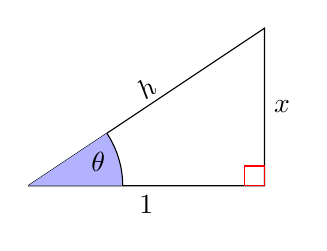
\begin{tikzpicture}
  \coordinate [] (C) at (-1.5cm,-1.cm);
  \coordinate [] (A) at (1.5cm,-1.0cm);
  \coordinate [] (B) at (1.5cm,1.0cm);
  \draw (C) -- node[above,label={[rotate = 35,label distance=-.25cm]:{$h$}}] {} (B) -- node[right] {$x$} (A) -- node[below] {$1$} (C);
  \draw [red](1.25cm,-1.0cm) rectangle (1.5cm,-0.75cm);
  \draw pic[draw,fill=blue!30,angle radius=1.2cm,"$\theta$" shift={(2mm,1mm)}] {angle=A--C--B};                      
\end{tikzpicture}
\end{document}